\documentclass[aspectratio=169]{beamer}
\usetheme{Madrid}
\beamertemplatenavigationsymbolsempty
\usepackage[utf8]{inputenc}
\usepackage[brazilian]{babel}
\usepackage{pmboxdraw}
\usepackage{longtable}
\usepackage{multirow}
\usepackage{listings}
\lstset{
    %frame=tb,
    aboveskip=3mm,
    belowskip=3mm,
    showstringspaces=false,
    basicstyle={\small\ttfamily},
    numbers=none,
    breaklines=true,
    breakatwhitespace=true,
    tabsize=4
}

\setbeamertemplate{footline}{
    \leavevmode
    \hbox{\begin{beamercolorbox}[wd=.175\paperwidth,ht=2.5ex,dp=1.125ex,leftskip=.3cm plus1fill,rightskip=.3cm]{author in head/foot}
        \usebeamerfont{title in head/foot}\insertshorttitle
    \end{beamercolorbox}
    \begin{beamercolorbox}[wd=.825\paperwidth,ht=2.5ex,dp=1.125ex,leftskip=.3cm,rightskip=.3cm plus1fil]{title in head/foot}
        \usebeamerfont{institute in head/foot}\insertinstitute
    \end{beamercolorbox}}
    \vskip0pt
}
\makeatother

\AtBeginSection[]{
    {
    \setbeamercolor{background canvas}{bg=beamer@blendedblue}
    \begin{frame}
    \vfill
    \centering
    \begin{beamercolorbox}[sep=8pt,center,shadow=false,rounded=true]{title}
        \usebeamerfont{title}\Huge\insertsectionhead\par%
    \end{beamercolorbox}
    \vfill
    \end{frame}
    }
}

\AtBeginSubsection[]{
    \begin{frame}
    \vfill
    \centering
    \begin{beamercolorbox}[sep=8pt,center,shadow=true,rounded=true]{title}
        \usebeamerfont{title}\insertsubsectionhead\par%
    \end{beamercolorbox}
    \vfill
    \end{frame}
}

\title{RISC-V SiMPLE}
\subtitle{Projeto e Desenvolvimento de processadores RISC-V com a \textit{ISA RV32IMF} usando as microarquiteturas Uniciclo, Multiciclo e \textit{Pipeline} em \textit{FPGA}}
\author{Arthur Matos}
\institute{Universidade de Brasília - UnB}
\date{26 de maio de 2021}

\makeatletter


\begin{document}

\begin{frame}
\titlepage
\end{frame}

%\begin{frame}
    %\tableofcontents
%\end{frame}

\section{Motivação e Objetivos}
    \begin{frame}
        \frametitle{Motivação e Objetivos}
        \vfill
        {}
        \vfill
    \end{frame}

\section{Revisão Teórica}
    \subsection{Arquitetura de computadores}
    \begin{frame}
        \frametitle{Arquitetura de computadores}
        \vfill
        \begin{figure}[H]
        \centering
            \includegraphics[width=.9\textwidth,height=.9\textheight,keepaspectratio]{../images/ABasicComputer.png}
        \end{figure}
        \vfill
    \end{frame}

    \begin{frame}
        \frametitle{RISC vs CISC}
        \vfill
        {}
        \vfill
    \end{frame}

    \subsection{ISA RISC-V}
    \begin{frame}
        \vfill
        \frametitle{\textit{\textbf{ISA RISC-V}}}
        \begin{figure}[H]
        \centering
            \includegraphics[width=.9\textwidth,height=.9\textheight,keepaspectratio]{../images/riscv_logo.png}
        \end{figure}
        \vfill
    \end{frame}

    \begin{frame}
        \frametitle{Módulo Base}
        \vfill
        {Falar sobre módulo I32/64/128 e E}
        \vfill
    \end{frame}

    \begin{frame}
        \frametitle{Extensões da arquitetura}
        \vfill
        {}
        \vfill
    \end{frame}

    \begin{frame}
        \frametitle{Codificação do tamanho da instrução}
        \vfill
        \begin{figure}[H]
        \centering
            \includegraphics[width=.9\textwidth,height=.9\textheight,keepaspectratio]{../images/RV_InstructionLength.png}
        \end{figure}
        \vfill
    \end{frame}

    \begin{frame}
        \frametitle{Instruções de 32 \textit{bits}}
        \vfill
        \begin{figure}[H]
        \centering
            \includegraphics[width=.9\textwidth,height=.9\textheight,keepaspectratio]{../images/RV_Formats.png}
        \end{figure}
        \vfill
    \end{frame}

    \begin{frame}[fragile]
        \frametitle{Imediatos}
        \vfill
        \begin{lstlisting}
        .text

        ...

        addi    t0, zero, 404
        ...
        \end{lstlisting}
        \vfill
    \end{frame}

    \begin{frame}
        \frametitle{Formação dos imediatos em instruções tipo \textbf{I}}
        \vfill
        \begin{figure}[H]
        \centering
            \includegraphics[width=.9\textwidth,height=.9\textheight,keepaspectratio]{../images/RV_I_Imm.png}
        \end{figure}
        \vfill
    \end{frame}

    \begin{frame}
        \frametitle{Formação dos imediatos em instruções tipo \textbf{S}}
        \vfill
        \begin{figure}[H]
        \centering
            \includegraphics[width=.9\textwidth,height=.9\textheight,keepaspectratio]{../images/RV_S_Imm.png}
        \end{figure}
        \vfill
    \end{frame}

    \begin{frame}
        \frametitle{Formação dos imediatos em instruções tipo \textbf{B}}
        \vfill
        \begin{figure}[H]
        \centering
            \includegraphics[width=.9\textwidth,height=.9\textheight,keepaspectratio]{../images/RV_B_Imm.png}
        \end{figure}
        \vfill
    \end{frame}

    \begin{frame}
        \frametitle{Formação dos imediatos em instruções tipo \textbf{U}}
        \vfill
        \begin{figure}[H]
        \centering
            \includegraphics[width=.9\textwidth,height=.9\textheight,keepaspectratio]{../images/RV_U_Imm.png}
        \end{figure}
        \vfill
    \end{frame}

    \begin{frame}
        \frametitle{Formação dos imediatos em instruções tipo \textbf{J}}
        \vfill
        \begin{figure}[H]
        \centering
            \includegraphics[width=.9\textwidth,height=.9\textheight,keepaspectratio]{../images/RV_J_Imm.png}
        \end{figure}
        \vfill
    \end{frame}

    \subsection{Organização de computadores}
    \begin{frame}
        \frametitle{Organização de computadores}
        \vfill
        \begin{figure}[H]
        \centering
            \includegraphics[width=.9\textwidth,height=.9\textheight,keepaspectratio]{../images/singlecycle_generic.png}
        \end{figure}
        \vfill
    \end{frame}

    \begin{frame}
        \frametitle{Alguns conceitos de microarquiteturas}
        \vfill
        \begin{itemize}
            \item Uniciclo
            \item Multiciclo
            \item \textit{Pipeline}
            \item Superescalar
            \item \textit{Out-of-Order Execution}
        \end{itemize}
        \vfill
    \end{frame}

    \subsection{Representação de \textit{hardware}}
    \begin{frame}
        \frametitle{Representação de \textit{hardware}}
        \vfill
        \begin{itemize}
            \item Programação visual
            \item Linguagens de descrição de \textit{hardware} (\textit{HDL})
            \begin{itemize}
                \item \textit{Verilog}
                \item \textit{VHDL}
            \end{itemize}
            \item Síntese de alto nível (\textit{HLS})
            \begin{itemize}
                \item \textit{C++}
                \item \textit{Matlab}
            \end{itemize}
        \end{itemize}
        \vfill
    \end{frame}

    \subsection{Síntese de \textit{hardware}}
    \begin{frame}
        \frametitle{Sintetizando projetos em \textit{HDL}}
        \begin{figure}[H]
        \centering
            \includegraphics[width=.9\textwidth,height=.8\textheight,keepaspectratio]{../images/quartus/quartus.png}
        \end{figure}
        \vfill
    \end{frame}

    \subsection{\textit{FPGAs}}
    \begin{frame}
        \frametitle{\textit{Field Programmable Logic Arrays}}
        \vfill
        \begin{block}{Arquitetura genérica de uma \textit{FPGA}}
        \begin{figure}[H]
            \begin{subfigure}
            \centering
                \includegraphics[width=.45\textwidth,height=.5\textheight,keepaspectratio]{../images/fpga_architecture_abstraction_-_olin_college.jpg}
            \end{subfigure}
            \begin{subfigure}
            \centering
                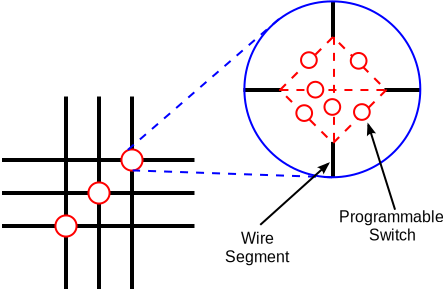
\includegraphics[width=.45\textwidth,height=.5\textheight,keepaspectratio]{../images/switch_box_wikimedia.png}
            \end{subfigure}
        \end{figure}
        \end{block}
        \vfill
    \end{frame}

    \begin{frame}
        \frametitle{\textit{FPGA Altera Cyclone V}}
        \vfill
        \begin{block}{Arquitetura da \textit{FPGA Altera Cyclone V}}
        \begin{figure}[H]
            \begin{subfigure}
            \centering
                \includegraphics[width=.5\textwidth,height=.5\textheight,keepaspectratio]{../images/altera_cyclone_v_soc_architectural_downscale.jpg}
            \end{subfigure}
            \begin{subfigure}
            \centering
                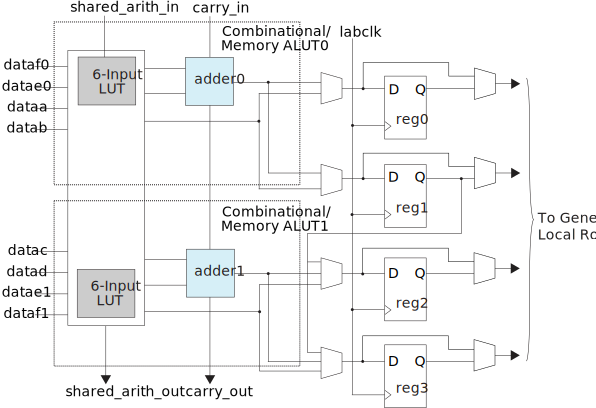
\includegraphics[width=.4\textwidth,height=.5\textheight,keepaspectratio]{../images/intel_alm_high_level.png}
            \end{subfigure}
        \end{figure}
        \end{block}
        \vfill
    \end{frame}

    \subsection{Estado da Arte}
    \begin{frame}
        \frametitle{O Estado da Arte da \textit{ISA RISC-V}}
        \vfill
        {}
        \vfill
    \end{frame}

\section{Sistema Proposto}
    \begin{frame}[fragile]
        \frametitle{Organização do projeto}
        \footnotesize{
        \begin{columns}
            \column{.5\textwidth}
            \begin{verbatim}
    ┌─ core
    ├─ doc
    ├─ project
    ├─ system
    ├─ test
    ├─ tools
    ├─ vendor
    ├─   .gitignore
    ├─   inst_decode.sh
    ├─   LICENSE
    ├─   make.sh
    ├─   gtkwave.sh
    ├─   rars.sh
    └─   README.md
        \end{verbatim}
        \vfill
        \column{.5\textwidth}
        \begin{verbatim}
   core
   ├─ clock
   ├─ memory
   ├─ misc
   ├─ peripherals
   ├─ risc_v
   │  ├─ CPU.v
   │  ├─ Control_*.v
   │  ├─ Datapath_*.v
   │  └─ ...
   ├─ config.v
   ├─ default_data.mif
   ├─ default_framebuffer.mif
   ├─ default_text.mif
   ├─ fpga_top.sdc
   └─ fpga_top.v
        \end{verbatim}
        \vfill
        \end{columns}}
    \end{frame}

    \subsection{Implementação dos \textit{soft-cores}}
    \begin{frame}
        \frametitle{Uniciclo \textit{RV32I} e \textit{RV32IM}}
        \vfill
        \begin{figure}[H]
        \centering
            \includegraphics[width=.9\textwidth,height=.85\textheight,keepaspectratio]{../images/uarch_diagrams/singlecycle-RV32I-RV32IM.png}
        \end{figure}
        \vfill
    \end{frame}

    \begin{frame}
        \frametitle{Uniciclo \textit{RV32IMF}}
        \vfill
        \begin{figure}[H]
        \centering
            \includegraphics[width=.9\textwidth,height=.85\textheight,keepaspectratio]{../images/uarch_diagrams/singlecycle-RV32IMF.png}
        \end{figure}
        \vfill
    \end{frame}

    \begin{frame}
        \frametitle{Multiciclo \textit{RV32I} e \textit{RV32IM}}
        \vfill
        \begin{figure}[H]
        \centering
            \includegraphics[width=.95\textwidth,height=.9\textheight,keepaspectratio]{../images/uarch_diagrams/multicycle-RV32I-RV32IM.png}
        \end{figure}
        \vfill
    \end{frame}

    \begin{frame}
        \frametitle{Multiciclo \textit{RV32IMF}}
        \vfill
        \begin{figure}[H]
        \centering
            \includegraphics[width=.9\textwidth,height=.85\textheight,keepaspectratio]{../images/uarch_diagrams/multicycle-RV32IMF.png}
        \end{figure}
        \vfill
    \end{frame}

    \begin{frame}
        \frametitle{\textit{Pipeline} de 5 estágios \textit{RV32I} e \textit{RV32IM}}
        \vfill
        \begin{figure}[H]
        \centering
            \includegraphics[width=.99\textwidth,height=.85\textheight,keepaspectratio]{../images/uarch_diagrams/pipeline-RV32I-RV32IM.png}
        \end{figure}
        \vfill
    \end{frame}

    \begin{frame}
        \frametitle{\textit{Pipeline} de 5 estágios \textit{RV32IMF}}
        \vfill
        \begin{figure}[H]
        \centering
            \includegraphics[width=.99\textwidth,height=.85\textheight,keepaspectratio]{../images/uarch_diagrams/pipeline-RV32IMF.png}
        \end{figure}
        \vfill
    \end{frame}

    \subsection{Chamadas de sistema}
    \begin{frame}[fragile]
        \frametitle{Chamadas de sistema}
        \vfill
        \begin{lstlisting}
    # Inicio do programa
    .include "MACROS.s"

    # Dados do programa
    .data
        ...

    # Instrucoes do programa
    .text
        ...

    # Chamadas de sistema
    .include "SYSTEM.s"
        \end{lstlisting}
        \vfill
    \end{frame}

    \subsection{Ambiente de programação em \textit{assembly RISC-V}}
    \begin{frame}
        \frametitle{Programando para a \textit{ISA RISC-V}}
        \vfill
        \begin{figure}[H]
        \centering
            \includegraphics[width=.9\textwidth,height=.85\textheight,keepaspectratio]{../images/rars.png}
            \caption{\textit{IDE RARS}}
        \end{figure}
        \vfill
    \end{frame}

    \begin{frame}
        \frametitle{Simulação e depuração pelo \textit{RARS}}
        \vfill
        \begin{figure}[H]
        \centering
            \includegraphics[width=.9\textwidth,height=.85\textheight,keepaspectratio]{../images/rars_debug.png}
        \end{figure}
        \vfill
    \end{frame}

    \subsection{Execução dos programas na \textit{FPGA}}
    \begin{frame}
        \frametitle{Placa de desenvolvimento \textit{terasIC DE1-SoC}}
        \vfill
        \begin{figure}[H]
        \centering
            \includegraphics[width=.9\textwidth,height=.85\textheight,keepaspectratio]{../images/fpga/de1_soc_subs.png}
        \end{figure}
        \vfill
    \end{frame}

    \begin{frame}
        \frametitle{\textit{Frame} de vídeo da \textit{FPGA}}
        \vfill
        \begin{figure}[H]
        \centering
            \includegraphics[width=.9\textwidth,height=.85\textheight,keepaspectratio]{../images/osd/display.jpg}
        \end{figure}
        \vfill
    \end{frame}

    \begin{frame}
        \frametitle{Depuração do código pela \textit{FPGA}}
        \vfill
        \begin{figure}[H]
        \centering
            \includegraphics[width=.9\textwidth,height=.85\textheight,keepaspectratio]{../images/osd/display_osd.jpg}
        \end{figure}
        \vfill
    \end{frame}

    \subsection{Simulação de forma de onda}
    \begin{frame}
        \frametitle{Simulação de forma de onda pelo \textit{ModelSim}}
        \vfill
        \begin{figure}[H]
        \centering
            \includegraphics[width=.9\textwidth,height=.85\textheight,keepaspectratio]{../images/quartus/quartus_modelsim.png}
        \end{figure}
        \vfill
    \end{frame}

    \begin{frame}
        \frametitle{Visualização da forma de onda pelo \textit{GTKWave}}
        \vfill
        \begin{figure}[H]
        \centering
            \includegraphics[width=.9\textwidth,height=.85\textheight,keepaspectratio]{../images/gtkwave/random.png}
        \end{figure}
        \vfill
    \end{frame}

    \subsection{\textit{Scripts}}
    \begin{frame}
        \frametitle{\textit{Scripts} do projeto}
        \vfill
        \begin{itemize}
            \item \texttt{gtkwave.sh}
            \item \texttt{inst-decode.sh}
            \item \texttt{make.sh}
            \item \texttt{rars.sh}
        \end{itemize}
        \vfill
    \end{frame}

\section{Resultados}
    \subsection{Síntese dos \textit{soft-cores}}
    \begin{frame}
        \frametitle{\textit{Reports} do \textit{Quartus}}
        \vfill
        \begin{footnotesize}
        \begin{longtable}{cc|c|c|c|c|c|c|c|}
            \cline{3-9}
                                                                    &                               & ALMs  & Regs  & Pins  & Mem Bits  & DSPs  & PLLs  & Max Clk   \\
            \cline{2-9}
                                                                    & \multicolumn{1}{|c|}{Máximo}  & 32070 & XXXXX & 457   & 4065280   & 87    & 1     & 50MHz     \\
            \hline
            \endfirsthead
            \cline{3-9}
                                                                    &                               & ALMs  & Regs  & Pins  & Mem Bits  & DSPs  & PLLs  & Max Clk   \\
            \cline{2-9}
                                                                    & \multicolumn{1}{|c|}{Máximo}  & 32070 & XXXXX & 457   & 4065280   & 87    & 1     & 50MHz     \\
            \hline
            \endhead
            \multicolumn{1}{|c}{\multirow{3}{*}{{Uniciclo}}}        & \multicolumn{1}{|c|}{RV32I}   & 4123  & 3160  & 103   & 2805792   & 0     & 1     & 12.5MHz   \\*
            \cline{2-9}
            \multicolumn{1}{|c}{ }                                  & \multicolumn{1}{|c|}{RV32IM}  & 7047  & 3179  & 103   & 2805792   & 12    & 1     & 12.5MHz   \\*
            \cline{2-9}
            \multicolumn{1}{|c}{ }                                  & \multicolumn{1}{|c|}{RV32IMF} & 9411  & 5558  & 103   & 2853408   & 18    & 1     & 3.5Mhz    \\
            \hline
            \multicolumn{1}{|c}{\multirow{3}{*}{{Multiciclo}}}      & \multicolumn{1}{|c|}{RV32I}   & 4102  & 3444  & 103   & 2805792   & 0     & 1     & 25MHz     \\*
            \cline{2-9}
            \multicolumn{1}{|c}{ }                                  & \multicolumn{1}{|c|}{RV32IM}  & 6726  & 3471  & 103   & 2805792   & 12    & 1     & 25MHz     \\*
            \cline{2-9}
            \multicolumn{1}{|c}{ }                                  & \multicolumn{1}{|c|}{RV32IMF} & 9108  & 5737  & 103   & 2853408   & 18    & 1     & 25MHz     \\
            \hline
            \multicolumn{1}{|c}{\multirow{3}{*}{\textit{Pipeline}}} & \multicolumn{1}{|c|}{RV32I}   & 4605  & 4139  & 103   & 2805792   & 0     & 1     & 25MHz     \\*
            \cline{2-9}
            \multicolumn{1}{|c}{ }                                  & \multicolumn{1}{|c|}{RV32IM}  & 7376  & 4145  & 103   & 2805792   & 12    & 1     & 25MHz     \\*
            \cline{2-9}
            \multicolumn{1}{|c}{ }                                  & \multicolumn{1}{|c|}{RV32IMF} & 9750  & 6568  & 103   & 2853408   & 18    & 1     & 25MHz*    \\
            \hline
        \end{longtable}
        \end{footnotesize}
        \vfill
    \end{frame}

    \subsection{Visualização das formas de onda das \textit{ISAs RV32IMF}}
    \begin{frame}
        \frametitle{Visualização da forma de onda no Uniciclo}
        \vfill
        \begin{figure}[H]
        \centering
            \includegraphics[width=.95\textwidth,height=.85\textheight,keepaspectratio]{../images/gtkwave/gtkwave_uni.png}
        \end{figure}
        \vfill
    \end{frame}

    \begin{frame}
        \frametitle{Visualização da forma de onda no Multiciclo}
        \vfill
        \begin{figure}[H]
        \centering
            \includegraphics[width=.95\textwidth,height=.85\textheight,keepaspectratio]{../images/gtkwave/gtkwave_multi.png}
        \end{figure}
        \vfill
    \end{frame}

    \begin{frame}
        \frametitle{Visualização da forma de onda no \textit{Pipeline}}
        \vfill
        \begin{figure}[H]
        \centering
            \includegraphics[width=.95\textwidth,height=.85\textheight,keepaspectratio]{../images/gtkwave/gtkwave_pipe.png}
        \end{figure}
        \vfill
    \end{frame}

    \subsection{\textit{Benchmarks}}
    \begin{frame}
        \frametitle{Comparativo de desempenho das diferentes microarquiteturas}
        \vfill
        \begin{longtable}{cc|c|c|c|}
            \cline{3-5}
                                                                    &                               & RV32I       & RV32IM      & RV32IMF   \\
            \hline
            \endhead
            \multicolumn{1}{|c}{\multirow{2}{*}{{Uniciclo}}}        & \multicolumn{1}{|c|}{time}    & 0x0000001E  & 0x00000012  & 0x00000034 \\
            \cline{2-5}
            \multicolumn{1}{|c}{ }                                  & \multicolumn{1}{|c|}{clock}   & 12.5MHz     & 12.5MHz     & 3.5MHz \\
            \hline
            \multicolumn{1}{|c}{\multirow{2}{*}{{Multiciclo}}}      & \multicolumn{1}{|c|}{time}    & 0x00000048  & 0x0000002E  & 0x0000003D \\
            \cline{2-5}
            \multicolumn{1}{|c}{ }                                  & \multicolumn{1}{|c|}{clock}   & 25MHz       & 25MHz       & 25MHz \\
            \hline
            \multicolumn{1}{|c}{\multirow{2}{*}{\textit{Pipeline}}} & \multicolumn{1}{|c|}{time}    & 0x00000015  & 0x00000010  & erro \\
            \cline{2-5}
            \multicolumn{1}{|c}{ }                                  & \multicolumn{1}{|c|}{clock}   & 25MHz       & 25MHz       & 25MHz \\
            \hline
        \end{longtable}
        \vfill
    \end{frame}

\section{Conclusões}
    \begin{frame}
        \frametitle{Objetivos alcançados}
        \vfill
        \begin{itemize}
            \item Código simplificado;
            \item 8 das 9 implementações funcionam conforme o esperado;
            \item Adição e melhoria de ferramentas para o desenvolvimento de \textit{hardware} e \textit{software};
        \end{itemize}
        \vfill
    \end{frame}

    \begin{frame}
        \vfill
        \frametitle{Perspectivas futuras}
        {Trabalhos futuros podem tratar de:}
        \begin{itemize}
            \item Deixar a implementação do \textit{pipeline RV32IMF bug-free};
            \item Simplificar partes do projeto de \textit{hardware} para melhorar o desempenho do sistema;
            \item Implementar versões de 64 \textit{bits} do sistema;
            \item Implementar uma \textit{ISA} diferente utilizando a plataforma como base.
        \end{itemize}
        \vfill
    \end{frame}

    \subsection{Obrigado}

\end{document}

